\documentclass[11pt]{article}
\usepackage{fullpage}
\usepackage{graphics,epsfig,color}
\usepackage{wrapfig}

\usepackage{times}
\usepackage{setspace}
\usepackage{amsmath,amsthm,amssymb}
%\usepackage[ruled,vlined,linesnumbered]{algorithm2e}
\usepackage{qtree}
\usepackage{subfigure}
\usepackage{url}
\usepackage{tikz}


%for code from latexdraw
%\usepackage[usenames,dvipsnames]{pstricks}
%\usepackage{epsfig}
%\usepackage{pst-grad} % For gradients
%\usepackage{pst-plot} % For axes


\newtheorem{theorem}{Theorem}[section]
%\newtheorem{proposition}{Proposition}[theorem]
\newtheorem{corollary}{Corollary}[section]
\newtheorem{lemma}{Lemma}[section]
%\newtheorem{claim}{Claim}[section]
\newtheorem{problem}{Problem}
%\newtheorem{conjecture}{Conjecture}[section]
\newtheorem{definition}{Definition}[section]
\newtheorem{observation}{Observation}[section]
\newtheorem{example}{Example}[section]
\newtheorem{openproblem}{Open Problem}[section]
\newtheorem{fact}{Fact}[section]
%\newcommand{\qedsymb}{\hfill{\rule{2mm}{2mm}}}

\newcommand{\qedsymb}{\hfill{\rule{2mm}{2mm}}}
\newenvironment{proofsketch}{\begin{trivlist}
\item[\hspace{\labelsep}{\noindent Proof Sketch: }]
}{\qedsymb\end{trivlist}}



%the following few lines until usepackage{algorithm2e} is to avoid the
%conflicts of algorithm2e with other packages.
\makeatletter
\newif\if@restonecol
\makeatother
\let\algorithm\relax
\let\endalgorithm\relax
%\usepackage[ruled,vlined,linesnumbered]{algorithm2e}
\usepackage[ruled,vlined,linesnumbered]{algorithm2e}


%\newenvironment{proof}{\begin{trivlist}
%\item[\hspace{\labelsep}{\bf\noindent Proof: }]}{\qedsymb\end{trivlist}}
%\newcommand{\qed}{\hfill\rule{2mm}{2mm}}

\newcommand{\remove}[1]{}



%--------------------------------


\begin{document}

\begin{center}
  {\LARGE CSCD501 Homework3}

\bigskip 

{\Large Will Czifro}

\end{center}

\bigskip 

\begin{problem}[20 points]
\label{prob:1}
 In class, we analyzed that the false matching probability of the Karp-Rabin algorithm for
a binary sequence is no more than $\pi(nm)/\pi(I)$, where $n$ is the sequence size, $m$ is the pattern size, and $\pi(x)$ is
the number of positive prime numbers that are no larger than $x$. Now consider the case where the sequence and
the pattern are drawn from an alphabet of size $\sigma$. Can you analyze the false matching probably of the Karp-Rabin
algorithm for this general setting ? According to the result from your analysis, what is the false matching probability
if we set $I = n2m$ ?
\end{problem}



%---------------------------------------

\begin{problem}[25 points]
\label{prob:2}
 Draw the automata for the pattern alabama for pattern matching. You can assume the
alphabet where the sequence is drawn from is $\Sigma = {a, b, l, m}$. Explain which state is the “starting state” and which
state is the “acceptance state”.
\end{problem}



%---------------------------------------

\begin{problem}[30 points]
\label{prob:3}
Consider a sequence $S$ of size $n$ which is drawn from an alphabet $\Sigma = {0, 1,..., σ − 1}$. The
\textbf{0-order empirical entropy} of the sequence S is defined as

$$
H_0(S) = \sum_{i=0}^{\sigma-1} \frac{n_i}{n} log_2 \frac{n}{n_i}
$$

where $n_i$ is the number of copies of the character $i$ in $S$. Then, the \textbf{0-order empirical entropy compressed size} of $S$
is defined as $nH_0(S)$. \footnote{Clearly, the definition of the 0-order empirical entropy is also valid for a bit sequence where the alphabet is just ${0, 1}$.} %\newline

Now suppose you are given such a sequence $S$ and you create a wavelet tree for $S$. It’s easy to see that the wavelet
tree will have exactly $\sigma − 1$ internal nodes, because the wavelet tree is a full binary tree \footnote{A full binary tree is a binary tree where all non-leaf nodes have exactly two children.}. Recall that each internal
node in the wavelet tree has a bit sequence. Let’s name these $(\sigma − 1)$ bit sequences as $B_0, B_1,...,B_{\sigma-2}$.

Prove the following amazing claim is true, regardless of the shape of the wavelet tree:

$$
nH_0(S) = \sum_{i=0}^{\sigma-2}|B_i|H_0(B_i)
$$

where $|B_i|$ is the number of bits in the bit sequence $B_i$, $for i = 0, 1,..., \sigma − 1$. (This claim says a 0-order entropy
compression of all the bit sequences automatically gives a 0-order entropy compression of the original sequence $S$.)
Hint: use the inductive proof idea and play with the definition of the entropy. Note that any subtree of the wavelet
tree is also a wavelet tree for a subsequence (not of neighboring letters in the original sequence of course).

\end{problem}




\begin{problem}[25 points]
\label{prob:4}
Suffix array is another elegant data structure for sequence indexing and pattern matching.
The suffix array $SA[0, 1,...,n − 1]$ of a sequence $S[0, 1,...,n − 1]$ is a permutation of ${0, 1,...,n − 1}$, such that
all the suffixes of $S: S[SA[0],...,n − 1]$, $S[SA[1],...,n − 1]$,...,$S[SA[n − 1],...,n − 1]$ are in the ascending
lexicographic order.

Now suppose you are given the $BWT$ of the sequence $S$ as well as the location of the last character $S[n − 1] =' \$'$
in the $BWT$, can you use the $BWT$ to construct the suffix array of $S$ ? Explain your idea and give the pseudocode.
(Hint: use idea for reversing the $BWT$.)

\end{problem}


%---------------------------------------

\bigskip
\noindent{\bf Solution for Problem~\ref{prob:1}.}



%---------------------------------------

\bigskip
\noindent{\bf Solution for Problem~\ref{prob:2}.}



%---------------------------------------

\bigskip
\noindent{\bf Solution for Problem~\ref{prob:3}.}


\begin{center}
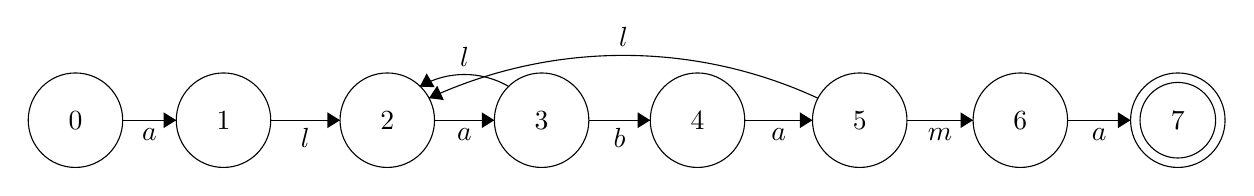
\begin{tikzpicture}[scale=0.2]
\tikzstyle{every node}+=[inner sep=0pt]
\draw [black] (5.2,-29.1) circle (3);
\draw (5.2,-29.1) node {$0$};
\draw [black] (14.6,-29.1) circle (3);
\draw (14.6,-29.1) node {$1$};
\draw [black] (25,-29.1) circle (3);
\draw (25,-29.1) node {$2$};
\draw [black] (34.8,-29.1) circle (3);
\draw (34.8,-29.1) node {$3$};
\draw [black] (44.7,-29.1) circle (3);
\draw (44.7,-29.1) node {$4$};
\draw [black] (55,-29.1) circle (3);
\draw (55,-29.1) node {$5$};
\draw [black] (65.2,-29.1) circle (3);
\draw (65.2,-29.1) node {$6$};
\draw [black] (75.2,-29.1) circle (3);
\draw (75.2,-29.1) node {$7$};
\draw [black] (75.2,-29.1) circle (2.4);
\draw [black] (8.2,-29.1) -- (11.6,-29.1);
\fill [black] (11.6,-29.1) -- (10.8,-28.6) -- (10.8,-29.6);
\draw (9.9,-29.6) node [below] {$a$};
\draw [black] (17.6,-29.1) -- (22,-29.1);
\fill [black] (22,-29.1) -- (21.2,-28.6) -- (21.2,-29.6);
\draw (19.8,-29.6) node [below] {$l$};
\draw [black] (28,-29.1) -- (31.8,-29.1);
\fill [black] (31.8,-29.1) -- (31,-28.6) -- (31,-29.6);
\draw (29.9,-29.6) node [below] {$a$};
\draw [black] (37.8,-29.1) -- (41.7,-29.1);
\fill [black] (41.7,-29.1) -- (40.9,-28.6) -- (40.9,-29.6);
\draw (39.75,-29.6) node [below] {$b$};
\draw [black] (47.7,-29.1) -- (52,-29.1);
\fill [black] (52,-29.1) -- (51.2,-28.6) -- (51.2,-29.6);
\draw (49.85,-29.6) node [below] {$a$};
\draw [black] (58,-29.1) -- (62.2,-29.1);
\fill [black] (62.2,-29.1) -- (61.4,-28.6) -- (61.4,-29.6);
\draw (60.1,-29.6) node [below] {$m$};
\draw [black] (68.2,-29.1) -- (72.2,-29.1);
\fill [black] (72.2,-29.1) -- (71.4,-28.6) -- (71.4,-29.6);
\draw (70.2,-29.6) node [below] {$a$};
\draw [black] (27.062,-26.971) arc (120.52999:59.47001:5.586);
\fill [black] (27.06,-26.97) -- (28.01,-27) -- (27.5,-26.13);
\draw (29.9,-25.7) node [above] {$l$};
\draw [black] (27.653,-27.703) arc (114.84615:65.15385:29.384);
\fill [black] (27.65,-27.7) -- (28.59,-27.82) -- (28.17,-26.91);
\draw (40,-24.48) node [above] {$l$};
\end{tikzpicture}
\end{center}



\end{document}




